\documentclass[addpoints]{exam}
\usepackage{amsmath, amsfonts}
\usepackage{geometry}
\usepackage{hyperref}
\usepackage{titling}
\usepackage{tikz} % Import the tikz package
\usetikzlibrary{automata} % Import library for drawing automata
\usetikzlibrary{positioning} % ...positioning nodes
\usetikzlibrary{arrows} % ...customizing arrows
\tikzset{node distance=2.5cm, % Minimum distance between two nodes. Change if necessary.
every state/.style={ % Sets the properties for each state
semithick,
fill=gray!10},
initial text={}, % No label on start arrow
double distance=2pt, % Adjust appearance of accept states
every edge/.style={ % Sets the properties for each transition
draw,
->,>=stealth', % Makes edges directed with bold arrowheads
auto,
semithick}}
% \let\epsilon\varepsilon


% Header and footer.
\pagestyle{headandfoot}
\runningheadrule
\runningfootrule
\runningheader{CS 212, Fall 2022}{HW 1: Regular Languages}{\theauthor}
\runningfooter{}{Page \thepage\ of \numpages}{}
\firstpageheader{}{}{}

\boxedpoints
\printanswers


\title{Homework 1: Regular Languages--Automata and Expressions}
\author{Finite Parser} % <=== replace with your team name
\date{CS 212 Nature of Computation\\Habib University\\Fall 2022}

\begin{document}
\maketitle

\begin{questions}

	\question For each of the languages specified below, provide the formal specification and the state diagram of a finite automaton that recognizes it.
	\begin{parts}
		\part[5] $L= \{w\in \{0,1\}^* \mid n_0(w)=2, n_1(w)\leq 5 \}$   where $n_x(w)$ denotes the counts of $x$s in $w$.
		\begin{solution}

			\begin{center}
				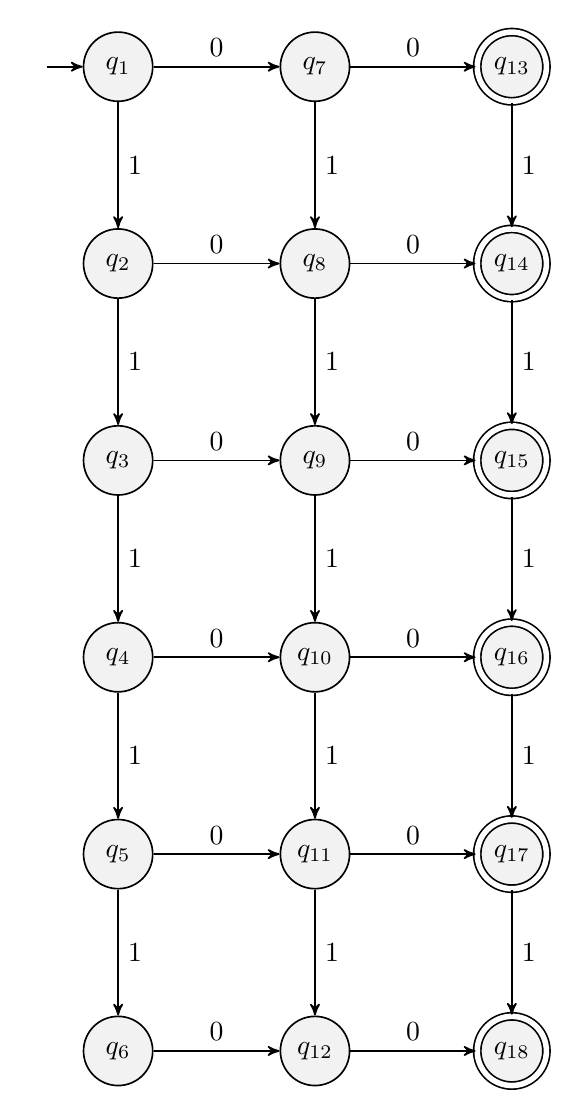
\begin{tikzpicture}
					\node[state, initial] (q1) {$q_1$};
					\node[state, below of=q1] (q2) {$q_2$};
					\node[state, below of=q2] (q3) {$q_3$};
					\node[state, below of=q3] (q4) {$q_4$};
					\node[state, below of=q4] (q5) {$q_5$};
					\node[state, below of=q5] (q6) {$q_6$};

					\node[state, right of=q1] (q7) {$q_7$};
					\node[state, right of=q2] (q8) {$q_8$};
					\node[state, right of=q3] (q9) {$q_9$};
					\node[state, right of=q4] (q10) {$q_{10}$};
					\node[state, right of=q5] (q11) {$q_{11}$};
					\node[state, right of=q6] (q12) {$q_{12}$};

					\node[state, accepting, right of=q7] (q13) {$q_{13}$};
					\node[state, accepting, right of=q8] (q14) {$q_{14}$};
					\node[state, accepting, right of=q9] (q15) {$q_{15}$};
					\node[state, accepting, right of=q10] (q16) {$q_{16}$};
					\node[state, accepting, right of=q11] (q17) {$q_{17}$};
					\node[state, accepting, right of=q12] (q18) {$q_{18}$};

					\draw (q1) edge node {$0$} (q7);
					\draw (q1) edge node {$1$} (q2);
					\draw (q2) edge node {$0$} (q8);
					\draw (q2) edge node {$1$} (q3);
					\draw (q3) edge node {$0$} (q9);
					\draw (q3) edge node {$1$} (q4);
					\draw (q4) edge node {$0$} (q10);
					\draw (q4) edge node {$1$} (q5);
					\draw (q5) edge node {$0$} (q11);
					\draw (q5) edge node {$1$} (q6);
					\draw (q6) edge node {$0$} (q12);

					\draw (q7) edge node {$0$} (q13);
					\draw (q7) edge node {$1$} (q8);
					\draw (q8) edge node {$0$} (q14);
					\draw (q8) edge node {$1$} (q9);
					\draw (q9) edge node {$0$} (q15);
					\draw (q9) edge node {$1$} (q10);
					\draw (q10) edge node {$0$} (q16);
					\draw (q10) edge node {$1$} (q11);
					\draw (q11) edge node {$0$} (q17);
					\draw (q11) edge node {$1$} (q12);
					\draw (q12) edge node {$0$} (q18);

					\draw (q13) edge node {$1$} (q14);
					\draw (q14) edge node {$1$} (q15);
					\draw (q15) edge node {$1$} (q16);
					\draw (q16) edge node {$1$} (q17);
					\draw (q17) edge node {$1$} (q18);
				\end{tikzpicture}
			\end{center}
		\end{solution}

		\newpage

		\part[5] $(((00)^*(11))\cup 01)^*$.
		\begin{solution}

			\begin{center}
				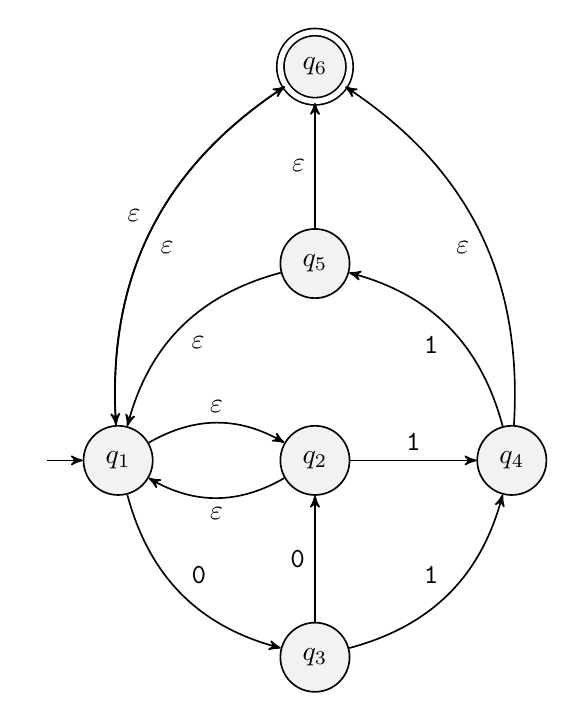
\begin{tikzpicture}
					\node[state, initial] (q1) {$q_1$};
					\node[state, right of=q1] (q2) {$q_2$};
					\node[state, below of=q2] (q3) {$q_3$};
					\node[state, right of=q2] (q4) {$q_4$};
					\node[state, above of=q2] (q5) {$q_5$};
					\node[state, accepting, above of=q5] (q6) {$q_6$};

					% \draw (q1) edge[loop above] node {\tt 0} (q1);
					\draw (q1) edge[bend left] node {\tt $\varepsilon$} (q2);
					\draw (q1) edge[bend right] node {\tt 0} (q3);

					\draw (q2) edge[bend left] node {\tt $\varepsilon$} (q1);
					\draw (q2) edge node {\tt 1} (q4);

					\draw (q3) edge node {\tt 0} (q2);
					\draw (q3) edge[bend right] node {\tt 1} (q4);

					\draw (q4) edge[bend right] node {\tt 1} (q5);

					\draw (q5) edge node {\tt $\varepsilon$} (q6);
					\draw (q5) edge[bend right] node {\tt $\varepsilon$} (q1);

					\draw (q4) edge[bend right] node {\tt $\varepsilon$} (q6);
					\draw (q1) edge[bend left] node {\tt $\varepsilon$} (q6);
					\draw (q6) edge[bend right] node {\tt $\varepsilon$} (q1);
				\end{tikzpicture}
			\end{center}

		\end{solution}
	\end{parts}

	Please see \href{https://www3.nd.edu/~kogge/courses/cse30151-fa17/Public/other/tikz_tutorial.pdf}{this guide} for help on drawing state diagrams.

	\newpage

	\question[5] Below is the transition table of a finite automaton. $\implies$ indicates the starting state, and $*$ indicates accepting states. Provide a regular expression for the language recognized by this automaton.
	\[
		\begin{array}{r|cc}
			           & 0         & 1          \\\hline
			p          & \{ q \}   & \emptyset  \\
			\implies q & \{ q \}   & \{ q, r \} \\
			*r         & \emptyset & \{ s \}    \\
			*s         & \emptyset & \emptyset  \\
		\end{array}
	\]
	\begin{solution}
		The following is the NFA made out of the delta function,
		\begin{center}
			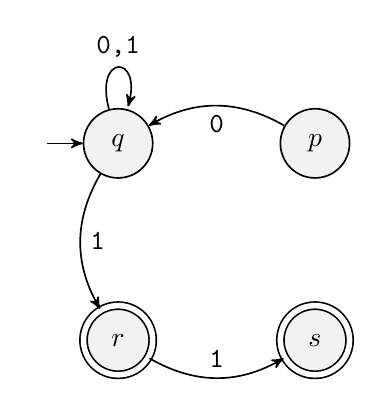
\begin{tikzpicture}
				\node[state, initial] (q) {$q$};
				\node[state, right of=q] (p) {$p$};
				\node[state, accepting, below of=q] (r) {$r$};
				\node[state, accepting, right of=r] (s) {$s$};

				\draw (p) edge[bend right] node {\tt 0} (q);
				\draw (q) edge[loop above] node {\tt 0,\tt 1} (q);
				\draw (q) edge[bend right] node {\tt 1} (r);
				\draw (r) edge[bend right] node {\tt 1} (s);
			\end{tikzpicture}
		\end{center}
		We can see that it accepts strings that have 1 or 11 at the end. So, the regular expression is \(\left(\Sigma^*\circ 1\right)\cup\left(\Sigma^*\circ 11\right)\).
	\end{solution}

	\question
	\begin{parts}
		\part[5] Suggest regular languages $L_1$ and $L_2$ over $\{0,1\}$ such that
		\begin{enumerate}
			\item $L_1\not\subseteq L_2$,
			\item $L_2\not\subseteq L_1$, and
			\item $(L_1\cup L_2)^* = L_1^* \cup L_2^*$
		\end{enumerate}
		\begin{solution}
			Let $L_1 = \{\epsilon\}$ and $L_2 = \{0\}$
			\\Then $L_1\not\subseteq L_2 \Longleftrightarrow  \{\epsilon\} \not\subseteq \{0\}$,
			\\and $L_2\not\subseteq L_1 \Longleftrightarrow  \{0\} \not\subseteq \{\epsilon\}$,
			\\So $(L_1\cup L_2)^* = ( \{\epsilon\} \cup \{0\})^* = \{\epsilon ,0\}^*$
			\\As $\{\epsilon\} \subset \{0\}^*$
			\\$\{\epsilon ,0\}^* = \{0\}^*$
				\\and $L_1^* \cup L_2^* = \{\epsilon\}^* \cup \{0\}^* =  \{\epsilon\} \cup \{0\}^* = \{0\}^*$
				\\Therefore $(L_1\cup L_2)^* = L_1^* \cup L_2^*$
			\begin{flushright}
				$\square$
			\end{flushright}
		\end{solution}

		\newpage

		\part[5] Prove or disprove whether condition 3 above holds for any regular languages, $L_1$ and $L_2$.
		\begin{solution}
			Let $L_1 = \{0\}$ and $L_2 = \{1\}$
			\\Then $L_1\not\subseteq L_2 \Longleftrightarrow  \{0\} \not\subseteq \{1\}$,
			\\and $L_2\not\subseteq L_1 \Longleftrightarrow  \{1\} \not\subseteq \{0\}$
			\\here $(L_1\cup L_2)^* \neq L_1^* \cup L_2^*$
			\\As we have $01 \in (L_1\cup L_2)^*$ and $01 \not\in  L_1^* \cup L_2^*$
			\\So we have $L_1 = \{0\}$ and $L_2 = \{1\}$ as counter examples, therefore the condition doesnt hold true for any regular languages $L_1$ and $L_2$.
			\begin{flushright}
				$\square$
			\end{flushright}
		\end{solution}
	\end{parts}

	\question[5] In class, we talked about the closure of the class, $A$, of regular languages under the union, concatenation, and star operations. In this question, we want to explore whether $A$ is also closed under intersection. That is, does the following hold?
	\[
		L_1\in A \land L_2\in A \implies L_1 \cap L_2\in A
	\]

	We want to go about it as follows. The expression, $L_1 \cap L_2$, can be transformed using DeMorgan's law to an equivalent one involving union, for which closure is known, and another operation. Show whether $A$ is closed under this operation, and use your result to argue about the closure of $A$ under intersection.
	\begin{solution}
		Let $L_1$ and $L_2$ be regualr languages, we show that $L_1 \cap L_2$ is also regular
		$$L_1 \cap L_2 = \overline{(\overline{(L_1 \cap L_2)})} = \overline{(\overline{L_1} \cup \overline{L_2})}$$
		For any language $L$, $\overline{L} = \Sigma^*/L$ so,
		$$\overline{(\overline{L_1} \cup \overline{L_2})} = \Sigma^*/(\Sigma^*/L_1 \cup \Sigma^*/L_2)$$
		We now show that if language $L$ is regular then $\Sigma^*/L$ is also regular
		\\For any regular language $L$ we have a DFA $M = (Q,\Sigma, \delta, q_0, F)$ that recognizes $L$, then we construct a machine $M'$ s.t. $M'$ recognizes $\Sigma^*/L$
		\\Let $M' = (Q,\Sigma, \delta, q_0, Q/F)$, as $M$ is a DFA then we know $\forall (q,a) \in Q \times \Sigma$ we have some transition through $\delta$, that is to say whatever state you are at, for ever symbol fot the alphabets that you input there you have some transition fot it in the DFA.
		\\So lets say we input $w \in \Sigma^*$ into $M$ then we have some state $q \in Q$ the machine will end up in, now if $q \in F$  then $q$ is an accept state for $M$ then as $q \not\in Q/F$, for $M'$ $q$ won't be an accept state so if $M$ accepts $w$ then $M'$ wont accept $w$.
		\\Likewise if $q \not\in F$  then $q$ is not an accept state for $M$ then as $q \in Q/F$, for $M'$ $q$ will be an accept state so if $M$ doesnt accepts $w$ then $M'$ accepts $w$.
		\\Therefore for all regular languages $L$, $\Sigma^*/L$ is also regular, so the class for regular languages is closed under complement operator.
		\\\\
		Now as class for regular langauges are closed under union operator and closed under complement operator,
		\\For regular languages $L_1$ and $L_2$, $\Sigma^*/L_1$ and $\Sigma^*/L_2$ are regular, then $\Sigma^*/L_1 \cup \Sigma^*/L_2$ is regular, then $\Sigma^*/(\Sigma^*/L_1 \cup \Sigma^*/L_2)$ is regular.
		\\Therefore $L_1 \cap L_2$ is regular.
		\\So the class of regular langauges are closed under intersection operator.
		\begin{flushright}
			$\square$
		\end{flushright}
	\end{solution}

	\question[5] We now want to explore the closure of the class, $A$, of regular languages under the operation, $mix$, which is defined as follows.
	\begin{itemize}
		\item Given strings, $u$ and $v$, both of length $n$, $\operatorname{mix}(u,v) = u_1v_1u_2v_2\ldots u_nv_n$.
		\item Given languages, $L_1$ and $L_2$, $\operatorname{mix}(L_1,L_2) = \{\operatorname{mix}(u,v) \mid u\in L_1, v\in L_2, |u| = |v|\}$.
	\end{itemize}
	Is $A$ closed under $mix$? Justify your answer.
	\begin{solution}
		Let $L_1, L_2 \in A$, then $\operatorname{mix}(L_1,L_2) = \{\operatorname{mix}(u,v) \mid u\in L_1, v\in L_2, |u| = |v|\}$
		\\We show $\operatorname{mix}(L_1,L_2) \in A$, we show this by induction we show that each $u \in L_1$ and $v \in L_2$, there exist a machine that recognize $\operatorname{mix}(u,v)$ then we can construct $M$ to recognize $\operatorname{mix}(L_1,L_2)$ just by taking unions of all such machines.
		\\\textbf{Base case:} $|u| = |v| = 1$
		\\Then $u = a$ and $v = b$, for some symbols $a,b \in \Sigma$ then,
		$$\operatorname{mix}(u,v) = ab = u\circ v \in A$$
		As for any language $u,v\in A \Rightarrow u\circ v \in A$
		\\So for  $|u| = |v| = 1$, $\operatorname{mix}(u,v) = u\circ v \in A$
		\\\textbf{Inductive Hypothesis:} for $|u| = |v| = k$, suppose $\operatorname{mix}(u,v) = u\circ v \in A$
		\\\textbf{Induction Step:} Let $|u| = |v| = k+1$
		\\let $u = u_1u_2...u_ku_{k+1} = u'u_{k+1}$, where $|u'| = k$ and $|u_{k+1}| = 1$
		\\let $v = v_1v_2...v_kv_{k+1} = v'v_{k+1}$, where $|v'| = k$ and $|v_{k+1}| = 1$
		\\Then $\operatorname{mix}(u,v) = \operatorname{mix}(u',v')\circ u_{k+1}v_{k+1}$
		\\As $|u'| = |v'| = k$, we from our inductive hypothesis we have $ \operatorname{mix}(u',v') \in A$ and as for $|u_{k+1}| = |v_{k+1}| = 1$, $u_{k+1}v_{k+1} =u_{k+1}\circ v_{k+1} \in A$
		\\And for any languages $U,V \in A$, $U \circ V \in A$ we have,
		$$\operatorname{mix}(u,v) = \operatorname{mix}(u',v')\circ u_{k+1}v_{k+1} \in A$$
		\\Therefore through the principle of mathematical induction we have that for any string $u \in L_1$ and $v\in L_2$ s.t. $|u| = |v| = n$ for any $n \in \mathcal{N}$, if $L_1, L_2 \in A$, then $\operatorname{mix}(u,v) \in A$
		\\Now,
		$$\operatorname{mix}(L_1,L_2) = \{\operatorname{mix}(u,v) \mid u\in L_1, v\in L_2, |u| = |v|\} = \bigcup\limits_{i=1}^{n} \left( \bigcup\limits_{r_1 \in L_1}\left( \bigcup\limits_{r_2 \in L_2}\operatorname{mix}(u_{r_1i},v_{r_2i}) \right)\right)$$
		Where each $u_{r_1i}$ is a string of size $i$ in $L_1$ and $v_{r_2i}$ is a string of size $i$ in $L_2$.
		\\As $\forall i \in \mathcal{N}, \; \operatorname{mix}(u_{r_1i},v_{r_2i}) \in A$,
		\\we have that each element in $ \operatorname{mix}(L_1,L_2) = \bigcup\limits_{i=1}^{n} \left( \bigcup\limits_{r_1 \in L_1}\left( \bigcup\limits_{r_2 \in L_2}\operatorname{mix}(u_{r_1i},v_{r_2i}) \right)\right)$ is in $A$ and for $\operatorname{mix}(L_1,L_2)$ we are just taking unions of all these elements in $A$ and as $A$ is closed under union, we have that $\operatorname{mix}(L_1,L_2) \in A$
		\\Therefore class of regular langauges is closed under $\operatorname{mix}$ operator
		\begin{flushright}
			$\square$
		\end{flushright}
	\end{solution}

\end{questions}

\end{document}

%%% Local Variables:
%%% mode: latex
%%% TeX-master: t
%%% End: